\section{Questionnaire selection (Sophie)}
\label{sec:questionnaire-sophie}
The key point that needs to be established via the questionnaire is whether the patient suffers from daytime sleepiness. However knowing about the patient’s weight can be useful to eliminate central sleep apnoea, and other questions about symptoms can be useful to reinforce diagnosis. 

\subsection{New vs. Pre-existing Questionnaire}
 There is a key decision between two options at this stage: to create a new questionnaire from scratch or to use a pre-existing questionnaire. A new questionnaire gives much more freedom as to what questions to ask in order to target particular symptoms and eliminate other disorders. It also allows for unique methods of analysis e.g. weighted questions rather than a simple threshold based on number of questions answered. Rigorous market research can be used to design the wording of the questions to maximise truthfulness and ease of interpretation, as well as number of questions and mechanism of answering. However this would be time consuming and an expert in question production is potentially needed. Data from patients would need to be collected via the questionnaire and other means in order to test its effectiveness, i.e. it could not be used as a retrospective study.

Using a pre-existing questionnaire allows for quicker set up time as there will either be data available in order to validate the questionnaire or it will have already been validated. Some questionnaires are within the doctor’s guideline so time can be saved during consultation if they are already performed. Named questionnaires are often recognised by doctors which saves them time checking the questions.

Given the time constraints and the access to data and skills, further investigation will look at pre-existing questionnaires. 
\subsection{Using app based questionnaires to increase patient truthfulness}
One of the benefits of performing questionnaires on the app rather than waiting for patients to attend an appointment is saving doctors time. However there is another benefit in the form of potentially increased truthfulness. 

Castelo-Branco et al found that patients tended to lie in order to look good, in the context of sexuality, when those involved had a strong interest in not giving a disappointing impression ~\cite{castelo2010patients}. Rogers looked at doctors’ trust in patients which is an indicator of suspected lying ~\cite{rogers2002there}. Ulterior motives were thought to have a significant influence on patients’ truthfulness. In the case of OSA there is a risk of patients playing down daytime sleepiness in order to avoid diagnosis if they wish to avoid having to contact the DVLA and their car insurance company and risk losing their license or insurance due to misunderstanding. There is also a case that patients may try and get a diagnosis in order to receive disability related financial support. However tricking a sleep test into thinking you have OSA would be challenging. 

\subsection{Questionnaires}
There are a number of questionnaires that have been used to assess diagnosis of OSA: some rely on a doctor to measure physical features, others use characteristic clinical features, others use patients’ interpretations of their symptoms, and the rest use combinations of the above. 

\begin{itemize}
\item Chung et al – STOP Questionnaire \\
Four questions on snoring, daytime sleepiness, witnessed apnoeas and blood pressure ~\cite{chung2008stop}.
\item Chung et al –STOPbang Questionnaire \\
This is an extension of the STOP questionnaire that adds four additional questions on BMI, age, neck circumference and gender. A threshold of 3 out of 8 is generally used to indicate OSA ~\cite{chung2012high}.
\item Chung et al – ASA \\
Three categories are used to ask questions: physical characteristics, observed sleep disturbances and tiredness. It uses falling into two or more of these categories as an indicator of OSA ~\cite{chung2008validation}.
\item Dixon et al \\
Looked at witnessed apnoeas, neck circumference and BMI. Study rather than a questionnaire ~\cite{dixon2003predicting}.
\item Flemons’ et al – Flemons’ screening tool \\
This is a 36 question screening tool for OSA that uses a differential method for diagnosis, asking questions about depression and chronic diseases as well as the more common questions on tiredness, snoring and driving behaviour. Uses a weighted score called SACS with a threshold to indicate OSA ~\cite{flemons1994likelihood}.
\item Kirby et al – Artificial Neural Nets \\
Uses 23 clinical variables including patient’s history, physical examination and patient reported sleepiness and smoking ~\cite{kirby1999neural}.
\item Kushida et al – Kushida Index \\
Complicated morphometric model, including BMI, neck circumference, palatal height and oral cavity measurements amongst others. Suffers from being too complicated to be administered accurately and being time consuming ~\cite{kushida1997predictive}.
\item Maislin et al \\
Model incorporates snoring, gasping at night, witnessed apnoeas, age, gender and BMI. Multiple logistic regressions were used to generate a multivariable apnoea risk register when compared to RDIs from polysomnographs. ROCs were used to test predictive ability ~\cite{dinges1995survey}.
\item Netzer et al – Berlin Questionnaire \\
Uses ten questions about snoring, witnessed apnoeas, daytime sleepiness, sleeping while driving, high blood pressure and BMI. Analysis is via simple scoring ~\cite{netzer1999using}.
\item Rosenthal and Dolan – Epworth Sleepiness Scale \\
A questionnaire using eight questions to assess sleepiness in different situations. Recommended by NHS guidelines ~\cite{rosenthal2008epworth}.
\item Tsai et al - Upper Airway Physical Examination Protocol \\
Looked at six parameters: three clinical symptoms; snoring, witnessed apnoeas and hypertension; and three measurable signs; cricomental space, pharyngeal grade and overbite (info on these to follow) ~\cite{tsai2003decision}.
\item Viner et al\\ 
Model incorporates snoring, BMI, age and gender. Used stepwise linear logistic regression ~\cite{viner1991history}.
\end{itemize}

\subsection{Narrowing Down the Studies}
There are too many questionnaires to look at all in detail. However given they are not all suitable for use in a mobile app they can be reduced in number and those that are more appropriate assessed. The Kushida Index and ASA questionnaire are complicated, which goes against the design specification, so can be discounted. Table \ref{table:questionnaire} shows the statistics the studies found for each questionnaire. A high negative predictive value is needed so the focus of more work will be on; Artificial Neural Net, UAPP and the STOPbang questionnaire. Epworth Sleepiness Scale will also be investigated for use in the app because it is part of the diagnostic pathway as laid out by the NHS.

\begin{table}[h]
\centering
\begin{tabular}{l l c c c c c c}
\toprule
Study&Test&n&Sens&Spec&Likelihood Ratio&NPV&PPV\\ \midrule
Chung et al&STOP&177&74&53&1.57&76&51\\ 
Chung et al&STOPbang&177&93&43&1.63&90&52\\ 
Chung et al&ASA&177&79&37&1.25&73&45\\ 
Dixon et al&&99&96&71&3.31&&\\ 
Flemons' et al&Flemons' screening tool&180&&&5.17&&81\\ 
Kirby et al&Artificial neural net&405&99&80&4.95&98&88\\ 
Kushida et al&Kushida index&300&98&100&large&88.5&100\\ 
Maislin et al&&427&60&&&&\\ 
Netzer et al&Berlin questionnaire&744&86&77&3.74&&89\\ 
Rosenthal&Epworth sleepiness scale&268&76&31&&&\\ 
Tsai et al&UAPP&75&40&96&10&100&95\\ 
Viner et al&&410&94&28&1.31&&\\ \bottomrule
\end{tabular}
\caption{Questionnaire Statistics based on an AHI \textgreater\ 15 threshold. n, number in the study; Sens, sensitivity (\%); Spec, specificity (\%); NPV, negative predictive value (\%); PPV, positive predictive value (\%).}
\label{table:questionnaire}
\end{table}
\subsection{Artificial Neural Net}
The 23 clinical variables which form the parameters for the neural network are shown in Table \ref{table:neural}. The patient would be aware of the demographics and social history information. However night time symptoms and bed partner observations would be more challenging and impossible for the patient to know about themselves in some cases. As regards past medical history, anthropometrics and the physical examination, in most cases the patient would not be able to self administer the questionnaire, negating its use.
\begin{table}[h]
\centering
\begin{tabular}{p{5cm} p{10cm}}
\toprule
Variables&Characteristics\\ \midrule
Demographics&Age, gender\\ 
Night time symptoms&Frequent awakening, experienced choking\\ 
Bed partner observations&Witnessed apnoeas, observed choking\\ 
Daytime symptoms&Reported excessive daytime sleepiness, Epworth sleepiness scale\\ 
Past medical history&Hypertension\\ 
Social history&Alcohol consumption, smoking in pack-yr\\ 
Anthropometrics&Height, weight, BMI, systolic BP ≥ 140, diastolic BP ≥ 90\\ 
Physical examination&Tonsillar enlargement, soft palate enlargement, crowding of the oral pharynx\\ 
Clinical score&Sum of the clinical scores for the binary categorical values (maximum score = 12)\\ \bottomrule
\end{tabular}
\caption{Patient Demographics and Clinical Features Used in the Neural Network of Prediction of OSA}
\label{table:neural}
\end{table} 

\subsection{Upper Airway Physical Examination Protocol}
This is only based on three features as shown in the flowchart(Figure \ref{fig:flowchart}: cricomental space, pharyngeal grade and overbite. All of these are physiological features hence their success at diagnosing OSA. However because they are physiological features there is a chance the patient would make significant errors while undertaking the readings. Cricomental space is the perpendicular distance from the cricomental line (which joins the cricoids cartilage in the neck to the chin) to the skin of the neck (see Figure \ref{fig:cricomental}), this is really hard to measure on yourself. Pharyngeal Grade measures how much the tonsils and other tissues at the back of the throat obscure the airway(see Figure \ref{fig:pharyngeal}). This is generally graded by eye and therefore might be possible for a patient to self assess. Overbite is where the top teeth are significantly in front of the bottom teeth; this is something a patient is generally aware of. When Tsai et al studied the UAPP as a diagnostic tool they had two different specialists assess the patients which reduces confidence in patients own ability to undertake such assessments. 

\begin{figure}[h]
\centering 
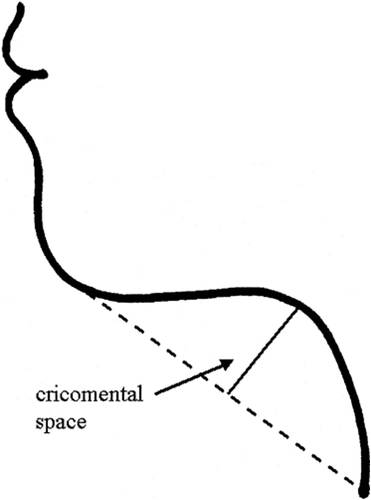
\includegraphics[width=0.2\textwidth]{drawings/cricomental}
\caption{Assessment of the cricomental space. Use a thin ruler to connect the cricoid cartilage to the inner mentum. The cricomental line is bisected, and the perpendicular distance to the skin of the neck is measured ~\cite{tsai2003decision}.}
\label{fig:cricomental}
\end{figure}
\begin{figure}[h]
\centering 
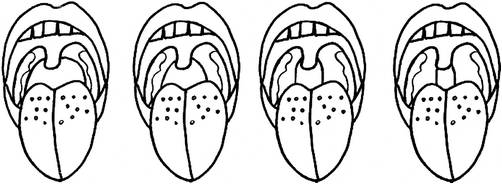
\includegraphics[width=0.4\textwidth]{drawings/pharyngeal}
\caption{Pharyngeal grading system. Class I = palatopharyngeal arch intersects at the edge of the tongue. Class II = palatopharyngeal arch intersects at 25\% or more of the tongue diameter. Class III = palatopharyngeal arch intersects at 50\% or more of the tongue diameter. Class IV = palatopharyngeal arch intersects at 75\% or more of the tongue diameter ~\cite{tsai2003decision}.}
\label{fig:pharyngeal}
\end{figure}
\begin{figure}[h]
\centering 
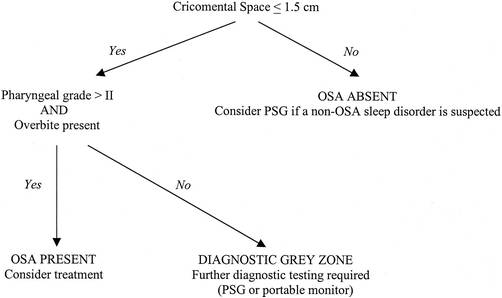
\includegraphics[width=0.5\textwidth]{drawings/flowchart}
\caption{A decision rule for diagnostic testing in OSA ~\cite{tsai2003decision}.}
\label{fig:flowchart}
\end{figure}


\subsection{STOPbang Questionnaire}
This questionnaire is based on eight questions to do with patients self reported symptoms. Each is answered with yes or no and the score is just a summation of the yes answers. Chung et al found that it was particularly good at distinguishing between severity of OSA, however as a simple diagnostic tool to find everyone who suffers it is relatively effective when used with a cut off of scoring 3 or above, with a probability of 93\% for detecting moderate OSA sufferers with AHI$\geq$15.
\begin{enumerate}
\item Snoring: Do you snore loudly (loud enough to be heard through closed doors)?
\item Tired: Do you often feel tired, fatigued, or sleepy during daytime?
\item Observed: Has anyone observed you stop breathing during your sleep?
\item Blood pressure: Do you have or are you being treated for high blood pressure?
\item BMI: BMI more than $35 \text{ kg} \text{m}^{−2}$?
\item Age: Age over 50 yr old?
\item Neck circumference: Neck circumference $>$ 40 cm?
\item Gender: Male?
\end{enumerate}

\subsection{Epworth Sleepiness Scale}
This is a tool for establishing how much the patient feels they suffer from daytime sleepiness. The patient is asked to say how likely they are to doze in eight situations with 0 being they would never doze, through slight and moderate to high chance of dozing given a 3. A cut off value of 8 has been proposed by Rosenthal and Dolan which gives a sensitivity of 76\% for an AHI $\geq$ 5. 
\begin{itemize}
\item Sitting and reading
\item Watching TV
\item Sitting, inactive in a public place (e.g. a theater or a meeting)
\item As a passenger in a car for an hour without a break
\item Lying down to rest in the afternoon when circumstances permit
\item Sitting and talking to someone
\item Sitting quietly after lunch without alcohol
\item In a car, while stopped for a few minutes in traffic
\end{itemize}

\subsection{Conclusion}
The STOPbang questionnaire and Epworth Sleepiness Scale are the only tests that a patient could reliably self administer, due to their shortness of length, ease to understand by a patient and ease to interpret by an algorithm. Both will be included in the app.
